\documentclass[letterpaper, 11pt]{article}

% package to adjust page margins
\usepackage[
	inner = 0.75in,
	outer = 0.75in, 
	top = 1in,
	bottom = 1in,
	bindingoffset = 0.0 cm
	]{geometry}

\usepackage[backend=biber]{biblatex}	% bibliography package using biber instead of bibtex
\usepackage{amsmath}	% provides enhancement of math printout structure 
\usepackage{amssymb}	% provides an extended symbol collection
\usepackage{comment}	% package to use comment block
\usepackage{sectsty}	% to change the style of section headers
\usepackage{fancyhdr}	% to have fancy headers for each page
\usepackage{graphicx}	% allows you to import images
\usepackage{float}	% allows the control of float positions
\usepackage{imakeidx} 	% to create index pages
\usepackage{afterpage}	% to place content (graphs mostly) in the next page
\makeindex[intoc] % creates index and toc

% allows for clickable references, also creates bookmarks that link to respective pages correctly
\usepackage[
	hidelinks, 
	bookmarksopen=true, 
	bookmarksnumbered=false, 
	bookmarksopenlevel=4,
	pdfview=Fit
	]{hyperref}

% List of macros
\newcommand{\pd}[2]{\frac{\partial#1}{\partial#2}}
\newcommand{\td}[2]{\frac{d#1}{d#2}}
\newcommand{\w}{w^{k}_{ij}}
\newcommand{\bpd}[2]{\dfrac{\partial#1}{\partial#2}}

\newcommand{\fint}{\int_{-\infty}^{\infty}} % integral with infinite limits
\newcommand{\sed}[2]{#2_{0}e^{2\pi if_{0}#1}e^{-#1/T} \theta (#1)} % SED function
\newcommand{\fsum}[1]{\sum_{#1 = -\infty}^{\infty}} % infinite sum
\newcommand{\spf}[2]{\Delta #1 \fsum{#2} \delta (#1 - #2 \Delta #1)} % sampling function
\newcommand{\fourier}[2]{\mathcal{F}_{#1}[#2]} % Fourier transform notation
\newcommand{\ifourier}[2]{\mathcal{F}_{#1}^{-1}[#2]} % inverse FT notation
\newcommand{\ft}[3]{\fint #2 e^{-2\pi i#3#1} d#1} % Fourier transform 
\newcommand{\ift}[3]{\fint #2 e^{2\pi i#1#3} d#1} % Inverse Fourier transform 
\newcommand{\conv}[4]{\fint #3(#2)#4(#1 - #2) d#2} % Convolution
\newcommand{\ssum}[1]{\sum_{#1 = 0}^{N - 1}} % sum from 0 to N-1
\newcommand{\dft}[3]{\ssum{#1} #2 e^{-2\pi i#3#1/N}} % DFT 
\newcommand{\idft}[3]{\frac{1}{N}\ssum{#1} #2 e^{2\pi i#3#1/N}} % Inverse DFT 
\newcommand{\dtft}[3]{\fsum{#1} #2 e^{-2\pi i#3#1}}

% Numbering equation and figure with section number
\numberwithin{equation}{section}
\numberwithin{figure}{section}
\numberwithin{table}{section}

% Centering section titles
\sectionfont{\centering}

% Adding bib file
\addbibresource{ft.bib}

\begin{document}
% Front cover page with title and name
\pdfbookmark[0]{Cover}{cover}
\begin{titlepage}
	\begin{center}
		% \vfill must have preceding text line
		\Huge{\bfseries Backpropagation}\vfill 
	\end{center}

	\begin{flushright}
		Sejin Nam\\
		University of Hawaii at Manoa
	\end{flushright}
\end{titlepage}

\begin{comment} % commenting out standard title page
\title{Fourier Transform}
\author{Sejin Nam}
\date{May 20}
\maketitle
\thispagestyle{empty}
\clearpage
\end{comment}

% page numbering in roman numerals
\pagenumbering{roman}

% Preface
\pdfbookmark[1]{Preface}{preface}
\section*{\centering Preface}
An \textbf{artificial neural network}\index{artificial neural network}, in short \textbf{ANN}\index{ANN}, is a machine learning model inspired by biological neurons found in our brains. As with any machine learning models, ANN model parameters must be optimized by training on large datasets in order to make good predictions. For ANN, \textbf{Gradient Descent}\index{Gradient Descent} (a generic optimization that tweaks parameters iteratively in order to minimize a cost function) is used to find those optimized parameters. In the context of ANN, \textbf{backpropagation}\index{backpropagation} is simply a Gradient Descent that computes the gradient of the network's errors with regard to every single model parameter efficiently. In this article, I will show my own derivation of backprogation of sequential ANN model. Not every variable is represented by conventional letters, and some variables and terms might have not even been defined before in machine learning community. It is implied that all materials that I did not come up with in this article cites the book by Aurelien Geron, Hands-on Machine Learning with Scikit-learn, Keras, and Tensorflow \cite{Geron}.
\cleardoublepage

% Table of Contents
\pdfbookmark[1]{Table of Contents}{toc}
\tableofcontents
\clearpage

% use fancyhdr
\pagestyle{fancy}

% First Section: artificial neural network
\pagenumbering{arabic}
\section{Artificial Neural Network}
An ANN, just like other machine learning models, takes a \textbf{model input} \(x\)\index{input!model} (a vector or column matrix containing scalars called \textbf{features}\index{feature}), which might have a \textbf{target}\index{target} (or label) value \(y\), and returns a \textbf{model output} \(h(x)\)\index{output!model} (\(h\) is called hypothesis or prediction function, and is often called interchangeably with a term model). The model output is either a scalar or a vector. We must first discuss what ANN is before we talk about backpropagation. And before we discuss what ANN is in detail, we should talk about the most fundamental component of ANN: Artificial neuron or neuron in short. 

% 1.1 Neuron
\subsection{Neuron}
A \textbf{neuron}\index{neuron}, in the context of ANN, is a mathematical function which takes an input vector and outputs a scalar (the input vector is a vector containing scalar outputs from other neurons). A neuron is graphically represented as a circle and scalars are represented as arrow sticks in the figure \ref{fig1}.

\afterpage{
\begin{figure}
	\centering
	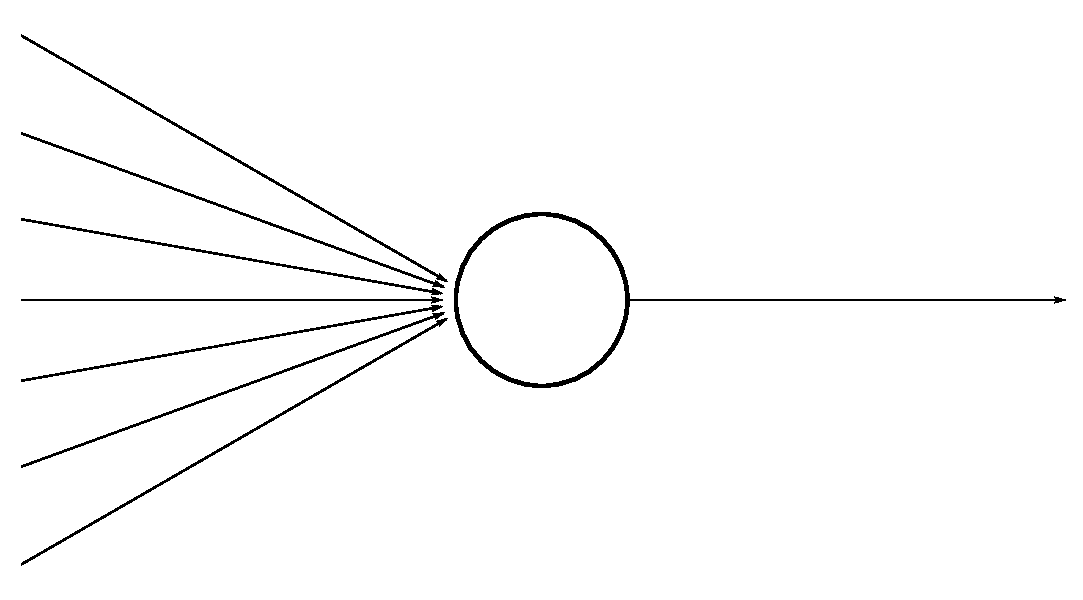
\includegraphics[height=4in]{neuron.eps}
	\caption{Graphical representation of an artificial neuron. Each arrow stick from right side represents a scalar (outputs from other neurons), and they collectively point to the left side of the neuron to represent an input vector. The right side arrow stick represents a neural output (scalar)}
	\label{fig1}
\end{figure}}

There are two special neurons called \textbf{bias neuron}\index{neuron!bias} and \textbf{input neuron}\index{neuron!input} which take no input vector. As their outputs, a bias neuron always returns 1 and an input neuron returns a feature value. Apart from those two neurons, a regular neuron is composed of connection weights (or weights for short), bias, matrix multiplication, and activation (transfer) function (how those components transform the input into the neural output is described below).

% 1.2 Neural variables
\subsection{Neural Variables}
Now let us define variables for a neuron that takes an input vector of \(M\) dimensions (\(M\) is always greater than 1).

\begin{itemize}
	\item \(a\) = input vector or input for short
	\item \(a_{i}\) = \(i\)-th component of \(a\)
	\item \(w\) = weight vector
	\item \(w_{j}\) = \(j\)-th component of \(w\) (weight for short) where \(1 \le j \le M - 1\)
	\item \(b\) = \(w_{M}\) = bias
	\item \(o\) = output scalar
	\item \(g\) = activation function
\end{itemize}

The indexing for vector and matrix is one-based in this article, i.e., indices of \(a\) and \(w\) start from 1 and all the indices are natural numbers. The input always contains 1 from a bias neuron, and in my definition it will always be the last element of the input, i.e., \(a_{M} = 1\).  The number of weights is one less than the number of elements of the input. 

% 1.3 Neuron output
\subsection{Neuron Output}
Let \textbf{a} be a column matrix of \(a\) and \textbf{w} be a row matrix of \(w\) and \(b\) for a neuron: 

\noindent\begin{minipage}{.5\linewidth}
\begin{align}
	\textbf{a}	&= 	\begin{bmatrix}
				a_{1}\\
				a_{2}\\
				\vdots\\
				a_{N-1}\\
				a_{N}
				\end{bmatrix}
\end{align}
\end{minipage}
\begin{minipage}{.5\linewidth}
\begin{align}
	\textbf{w}	&= 	\begin{bmatrix}
				w_{1} & w_{2} & \hdots & w_{N-1} & w_{N}
				\end{bmatrix}
\end{align}
\end{minipage}
\break

where \(N\) is a number of elements of the input, \(a_{N} = 1\), and \(w_{N} = b\). In this article, I call those matrices input and weight vector as well (in this case the number of elements of both is the same because of the bias term). The output value for the neuron is then:

\begin{align}
	o &= g(\textbf{w}\textbf{a})
\end{align}
The most typical activation function is ReLU:

\begin{equation}
	g(x) = \text{max}(0, x)
\end{equation}

% 1.4 Layer
\subsection{Layer}
In ANN, a \textbf{layer}\index{layer} is an exclusive set of neurons. There are three types of layers: input, hidden, and output. The \textbf{input layer}\index{layer!input} contains multiple input neurons and one bias neuron, and is the very first layer that an ANN starts with. The number of input neurons is exactly equal to the size of the model input \(x\), and each input neuron outputs distinctive feature values, i.e., no input neurons output the same feature value. The \textbf{hidden layer}\index{layer!hidden} contains multiple regular neurons and one bias neuron. The \textbf{output layer}\index{layer!output} contains multiple regular neurons and returns the final ouput of the ANN \(h(x)\), and this layer is the last layer of the neural network. A neuron in an output layer is called an \textbf{output neuron}\index{neuron!output}. Typically, regular neurons in the same layer have the same activation function and it is usually safe to assume that is always the case. In this article, activation functions for neurons in the same layer are the same. 

A layer, just like a neuron, returns an output, called \textbf{layer output}\index{output!layer} as a collection of output scalars from neurons in that layer. And such layer output can also be an input of a subsequent layer, called \textbf{layer input}\index{input!layer}. Such layer input provides its scalar values to form input vectors for neurons in that layer.

Now consider a hidden layer that contains \(N\) regular neurons which take the same input vector of \(M\) dimensions, \textbf{a}, from the preceding layer output (\(N\) is presumed to be at least 1). If the neurons have an activation function \(g\), then we can refine some of the neural variables above in the the following way:

\begin{itemize}
	\item \(w_{i}\) = weight vector for the \(i\)-th neuron where \(1 \le i \le N\)
	\item \(w_{ij}\) = \(j\)-th component of \(w_{i}\) where \(1 \le j \le M - 1\)
	\item \(b_{i}\) = \(w_{iM}\) = bias for the \(i\)-th neuron
	\item \textbf{W} = \(N \times M\) weight matrix (or \textbf{kernel}\index{kernel}) where \(\textbf{W}_{ij} = w_{ij}\)  
	\item \(o_{i}\) = \(g([\textbf{Wa}]_{i})\) = output scalar from the \(i\)-th neuron \(1 \le i \le N\)
	\item \(o_{N+1}\) = 1 = output scalar from the bias neuron
\end{itemize}

% 1.5 Sequential Model
\subsection{Sequential Model}
In a \textbf{sequential model}\index{model!sequential} of ANN, each hidden layer is stacked next to each other without branching (an ANN model that is not sequential is a \textbf{functional model}\index{model!functional}), starting from an input layer and ending with an output layer. And if an ANN contains a deep stack of hidden layers, it is called a \textbf{deep neural network}\index{deep neural network} (\textbf{DNN}\index{DNN}). In the 1990s, an ANN with more than two hidden layers was considered deep. Nowadays, it is common to see ANNs with hundreds of layers, so the definition of “deep” is quite blurred.

In a sequential model, the signal flows from one layer to another sequentially, meaning a layer, except for the input layer, takes a layer output from the preceding layer as its input. Also, clearly there should be at least two layers in any ANN, the first layer being an input layer and the last layer being an output layer. The figure \ref{fig2} is an example of a sequential neural network. In this article, only a sequential model case will be considered.

\afterpage{
\begin{figure}
	\centering
	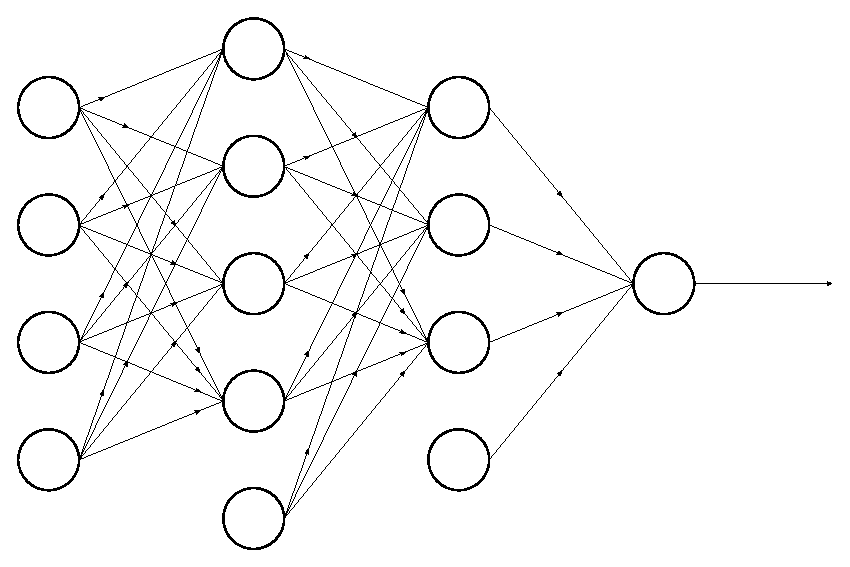
\includegraphics[height=4in]{sequential.eps}
	\caption{Graphical representation of a simple sequential model. The leftmost layer is the input layer and it has four neurons, the first three being input neurons and the last being a bias neuron. There are two hidden layers in this picture. The first hidden layer has five neurons and the second hidden layer has four neurons.  The last layer is the output layer (only one neuron) and returns the final output scalar of the model. A line with an arrow on it between two neurons represents connection. Notice the very last neurons of each hidden layer: they do not form any connections with neurons in the previous layers as those are bias neurons.}
	\label{fig2}
\end{figure}}

% 1.6 Dense Layer
\subsection{Dense Layer}
We say that two neurons are connected if one neuron takes an input vector that contains an output scalar from the other neuron as an element of the input. If every neuron except for the bias neuron in a layer is connected to every neuron in the previous layer, then the layer is called a \textbf{fully connected layer}\index{layer!fully connected} or a \textbf{dense layer}\index{layer!dense}(an input layer can never be fully connected as it takes no input). If every layer except for the input layer is fully connected in an ANN, then the ANN is called a \textbf{fully connected neural network}\index{neural network!fully connected}. The sequential neural network in the figure \ref{fig2} is a fully connected neural network. In this article, we will only consider a fully connected neural network model.

% 1.7 Neural Network Variables
\subsection{Neural Network Variables}
Consider a fully connected sequeltial ANN which contains \(L\) hidden layers. And suppose \(1 \le L\) for at least one hidden layer to be present. The model input \(x\) is fed into the network which then returns the model output \(h(x)\). Building upon the previously defined variables, let us define the following variables:

\begin{itemize}
	\item \(N_{0}\) = number of input neurons in the input layer = model input size
	\item \(x_{i}\) = \(i\)-th component of \(x\) where \(1 \le i < N_{0}\)
	\item \(o^{0}_{i}\) = \(x_{i}\) = output scalar from the \(i\)-th neuron in the input layer where \(1 \le i \le N_{0}\) 
	\item \(o^{0}_{N_{0}+1}\) = 1 = output scalar from the bias neuron in the input layer
	\item \(a^{k}\) = input vector for the \(k\)-th hidden layer where \(1 \le k \le L\)
	\item \(\textbf{a}_{k}\) = column matrix representation of \(a^{k}\)
	\item \(M_{k}\) = size or dimension of \(a^{k}\) 
	\item \(a^{k}_{i}\) = \(i\)-th component of \(a^{k}\) where \(1 \le i \le M_{k}\)
	\item \(N_{k}\) = number of regular neurons in the \(k\)-th hidden layer
	\item \(w^{k}_{i}\) = weight vector for the \(i\)-th neuron in the \(k\)-th hidden layer where \(1 \le i \le N_{k}\)
	\item \(w^{k}_{ij}\) = \(j\)-th component of \(w^{k}_{i}\) where \(1 \le j \le M_{k} - 1\)
	\item \(b^{k}_{i}\) = \(w^{k}_{iM_{k}}\) = bias for the \(i\)-th neuron in the \(k\)-th layer
	\item \(\textbf{W}_{k}\) = \(N_{k} \times M_{k}\) weight matrix of the \(k\)-th hidden layer where \([\textbf{W}_{k}]_{ij} = w^{k}_{ij}\)  
	\item \(\textbf{c}_{k} = \textbf{W}_{k}\textbf{a}_{k}\) = column matrix representation of weighted sums of \(a^{k}_{i}\) elements with \(w^{k}_{i}\) for indices \(i\) where \([\textbf{c}_{k}]_{i} = c^{k}_{i}\)
	\item \(g^{k}\) = activation function for the \(k\)-th hidden layer
	\item \(o^{k}_{i}\) = \(g^{k}(c^{k}_{i})\) = output scalar from the \(i\)-th neuron in the \(k\)-th hidden layer where \(1 \le i \le N_{k}\)
	\item \(o^{k}_{N_{k}+1}\) = 1 = output scalar from the bias neuron in the \(k\)-th hidden layer
	\item \(a^{L+1}\) = input vector for the output layer
	\item \(\textbf{a}_{L+1}\) = column matrix representation of \(a^{L+1}\)
	\item \(M_{L+1}\) = size or dimension of \(a^{L+1}\) 
	\item \(a^{L+1}_{i}\) = \(i\)-th component of \(a^{L+1}\) where \(1 \le i \le M_{L+1}\)
	\item \(N_{L+1}\) = number of neurons in the output layer = size of model output \(h(x)\)
	\item \(w^{L+1}_{i}\) = weight vector for the \(i\)-th neuron in the output layer where \(1 \le i \le N_{L+1}\)
	\item \(w^{L+1}_{ij}\) = \(j\)-th component of \(w^{L+1}_{i}\) where \(1 \le j \le M_{L+1} - 1\)
	\item \(b^{L+1}_{i}\) = \(w^{L+1}_{iM_{L+1}}\) = bias for the \(i\)-th neuron in the output layer
	\item \(\textbf{W}_{L+1}\) = \(N_{L+1} \times M_{L+1}\) weight matrix of the output layer where \([\textbf{W}_{L+1}]_{ij} = w^{L+1}_{ij}\)  
	\item \(\textbf{c}_{L+1} = \textbf{W}_{L+1}\textbf{a}_{L+1}\) = column matrix representation of weighted sums of \(a^{L+1}_{i}\) elements with \(w^{L+1}_{i}\) for indices \(i\) where \([\textbf{c}_{L+1}]_{i} = c^{L+1}_{i}\)
	\item \(\textbf{c}^{L+1}\) = \((\textbf{c}_{L+1})^{T}\) = transpose of \(\textbf{c}_{L+1}\)
	\item \(\sigma_{i}\) = activation function for the \(i\)-th output neuron
	\item \(h_{i}\) = \(\sigma_{i}(\textbf{c}_{L+1})\) = \(i\)-th element of model output \(h(x)\) where \(1 \le i \le N_{L+1}\)
\end{itemize}
As there should be at least one feature value in \(x\) and at least one regular neuron in a non-input layer, we know that 

\begin{equation}
	1 \le N_{k}
\end{equation}
for \(0 \le k \le L+1\). Since the considered model is sequential and fully connected, the entire collection of output scalars from a non-output layer forms an input vector for the subsequent layer. In other words, 

\begin{equation}
	o^{k-1}_{i} = a^{k}_{i}
\end{equation}
for \(1 \le k \le L+1\). Also it should be apparent that

\begin{equation}
	N_{k-1} + 1 = M_{k}\label{eq1.7}
\end{equation}
since \(N_{k-1}\) regular neurons (or input neurons) and one bias neuron all return output scalars that form the input vector \(a^{k}\).

The model \(h\) has model parameters in the output layer as its function parameters because its element is returned from an activation function that depends on \(\textbf{c}_{L+1}\) which is obtained by \(\textbf{W}_{L+1}\textbf{a}_{L+1}\). \(h\) also has model parameters in the last hidden layer as its function parameters because it depends on \(\textbf{a}_{L+1}\) that is obtained from an activation function that depends on \(\textbf{W}_{L}\textbf{a}_{L}\). You can use this induction to conclude that \(h\) has model parameters in every layer as its function parameters, and \(\textbf{a}^{k}\) depends on model parameters in layers that come before the \(k\)-th hidden layer (or the output layer if \(k = L+1\)) if \(1 < k\). 

If you inspect the definitions of activation function for a hidden and the output layer, you will notice that for the hidden layer, \(g\) depends on only one element of \textbf{c} whereas for the output layer, \(\sigma\) can depend on \textbf{c}. One example of \(\sigma\) that depends on \textbf{c} is softmax function:
\begin{equation}
	\sigma_{i}(\textbf{c}) = \frac{e^{c_{i}}}{\sum\limits^{N}_{j=1} e^{c_{j}}}  
\end{equation}
Even though nothing prevents activation function to depend on any variables, we will stick with the above case.

% Second Section: Backpropagation
\clearpage
\section{Backpropagation}
With a fully connected sequential neural network to consider, we can now discuss what backpropagation is in detail. For our model \(h\), weights \(\w\) are model parameters we want to optimize by training. For validation, \(L\), \(N_{k}\), \(g_{k}\) (with \(1 \le k \le L\)), and \(\sigma\) are hyperparameters to be tuned.

% 2.1 Cost Function
\subsection{Cost Function}
Let \(X\) be a collection of \(m\) input data, i.e., \(X = \{x^{1}, x^{2}, \dots, x^{m-1}, x^{m}\}\), and \(Y\) be a collection of targets for \(X\), i.e., \(Y =\{y^{1}, y^{2}, \dots, y^{m-1}, y^{m}\}\) (\(y^{i}\) is the target for \(x^{i}\)). The sizes of \(x\) and \(y\) are \(N_{0}\) and \(N_{L+1}\) respectively, and clearly \(X\) and \(Y\) have the same cardinality \(m\). Suppose the model is trained on those datasets. Then a cost function \(J\) of the model \(h\) is a function of \(X\) and \(Y\) (\(J(X,Y;h)\)). One example of \(J\) is cross entropy:

\begin{equation}
	J = -\frac{1}{m} \sum_{i=1}^{m} \sum_{j=1}^{N_{L+1}}y^{i}_{j}\ln(h^{i}_{j})	
\end{equation}
Where \(h^{i} = h(x^{i})\). Now let \(W\), \(G\), \(N\) be collections of \(\w\), \(g_{k}\), \(N_{k}\) of the model respectively. Since those are function parameters of \(h\), including \(L\), they are function parameters of \(J\) as well, i.e., (\(J(X,Y;h)\) = \(J(X,Y;W,G,N,L)\). Since backpropagation is a gradient descent that optimizes the model parameters, we can let \(W\) be a variable of \(J\) and let \(X\) and \(Y\) be the function parameters instead, i.e., \(J(W;X,Y,G,N,L) = J(W)\). The training is simply finding \(W\) that minimizes \(J\) (you can add an additional term to regularize the cost function, but in this article no regularization is considered as it is not relevant to the discussion of backpropagation). 

% 2.2 Gradient Descent
\subsection{Gradient Descent}
With the cost function \(J\), we can update \(W\) iteratively by the following assignment operation until \(J\) is miminized (gradient descent method): 

\begin{equation}
	w^{k}_{ij} \leftarrow  w^{k}_{ij} - \eta \pd{J}{\w}\label{gradient}
\end{equation}
Where \(\eta\) is called \textbf{learning rate}\index{learning rate}. All of \(\w\) must be iterated before the next iteration. For each iteration, you can also update the learning rate, but in this article the learning rate is kept constant. 

% 2.3 Partial Derivative of J
\subsection{Partial Derivative of J}
Let us evaluate the partial derivative term in \ref{gradient}. First we know that \(J\) contains \(m \times N_{L+1}\) many \(h\) terms that depend on weights. Thus:

\begin{equation}
	\pd{J}{\w} = \sum_{p=1}^{m}\sum_{q=1}^{N_{L+1}} \pd{J}{h^{p}_{q}}\pd{h^{p}_{q}}{\w}\label{eq2.3}
\end{equation}

\(\partial{J}/\partial{h^{p}_{q}}\) term expression is specific to the choice of the cost function, so we will leave it as it is. For \(\partial{h^{p}_{q}}/\partial{\w}\), we can further evaluate. Since \ref{eq2.3} deals with \(m\) many \(x\), \(h\) term has a superscript \(p\) for \(x^{p}\).  For simplicity, we will evaluate the second derivative term with a general \(x\) so we do not have to be concerned with the superscript \(p\), i.e., \(\partial{h_{q}}/\partial{\w}\) notation will be used. Now let us evaluate \(\partial{h_{q}}/\partial{\w}\):
\begin{equation}
	\begin{aligned}[b]
		\pd{h_{q}}{\w} 
		&= \pd{\sigma_{q}}{\w} \\ 
		&= \sum_{r=1}^{N_{L+1}}\pd{\sigma_{q}}{c^{L+1}_{r}}\pd{c^{L+1}_{r}}{\w}\\
		&= \pd{\sigma_{q}}{\textbf{c}^{L+1}}\pd{\textbf{c}_{L+1}}{\w}\label{eq2.4}
	\end{aligned}
\end{equation}
where 
\begin{equation}
	\pd{\sigma_{q}}{\textbf{c}^{L+1}} = 
		\begin{bmatrix}
			\bpd{\sigma_{q}}{c^{L+1}_{1}}&
			\bpd{\sigma_{q}}{c^{L+1}_{2}}&
			\hdots&
			\bpd{\sigma_{q}}{c^{L+1}_{N^{L+1}-1}}&
			\bpd{\sigma_{q}}{c^{L+1}_{N^{L+1}}}
		\end{bmatrix}
\end{equation}
And we know that 
\begin{equation}
		c^{l}_{r}
		= \sum_{s=1}^{N_{l-1}+1}w^{l}_{rs}a^{l}_{s}\label{eq2.5}
\end{equation}
where \(1 \le l \le L+1\) and the number of summands is determined by \ref{eq1.7}. The partial derivative of \ref{eq2.5} with respect to \(\w\) is then:

\begin{equation}
	\pd{c^{l}_{r}}{\w}
	= \sum_{s=1}^{N_{l-1}+1}(\pd{w^{l}_{rs}}{\w}a^{l}_{s}+w^{l}_{rs}\pd{a^{l}_{s}}{\w})\label{eq2.6}
\end{equation}
where we know \(a^{l}\) depends on weights only in layers that come before the \(l\)-th hidden layer (or output layer if \(l = L+1\)) if \(1 < l\). Thus, \ref{eq2.6} is simply 0 if \(l < k\). 

If \(l = k\), then:
\begin{equation}
	\begin{aligned}[b]
		\pd{c^{l}_{r}}{\w}
		&= \sum_{s=1}^{N_{l-1}+1} \delta_{ri}\delta_{sj}a^{k}_{s}\\
		&= \delta_{ri}a^{k}_{j}
	\end{aligned}
\end{equation}
where Kronecker delta relation is used:
\begin{equation}
	\begin{aligned}[b]
		\delta_{ij}	&=\begin{cases}
				1, 	&\text{if } i=j\\
				0,	&\text{otherwise}
		\end{cases}
	\end{aligned}
\end{equation}
In other words,
\begin{equation}
	\begin{aligned}[b]
		\pd{\textbf{c}_{k}}{\w}
		&= a^{k}_{j}	\begin{bmatrix}
				\delta_{1i}\\
				\delta_{2i}\\
				\vdots\\
				\delta_{N_{k}-1,i}\\
				\delta_{N_{k}i}
				\end{bmatrix}
	\end{aligned}
\end{equation}
If \(k < l\), then:

\begin{equation}
	\begin{aligned}[b]
		\pd{c^{l}_{r}}{\w} 
		&= \sum_{s=1}^{N_{l-1}+1}w^{l}_{rs}\pd{a^{l}_{s}}{\w}
			&&(\text{from }\ref{eq2.6}\text{ with }\pd{w^{l}_{rs}}{\w}=0)\\
		&= \sum_{s=1}^{N_{l-1}}w^{l}_{rs}\pd{o^{l-1}_{s}}{\w}
			&&(a^{l}_{s} = o^{l-1}_{s}\text{ and } o^{l-1}_{N_{l-1}+1} = 1)\\
		&= \sum_{s=1}^{N_{l-1}}w^{l}_{rs}\td{g^{l-1}}{c^{l-1}_{s}}\pd{c^{l-1}_{s}}{\w}
			&&(o^{l-1}_{s} = g^{l-1}(c^{l-1}_{s})\text{ with chain rule})\label{eq2.9}
	\end{aligned}
\end{equation}

If we define \(N_{l}\) by \(N_{l-1}\) matrix \(\textbf{S}_{l-1}\) such that:
\begin{equation}
	[\textbf{S}_{l-1}]_{rs} = w^{l}_{rs}\td{g^{l-1}}{c^{l-1}_{s}}
\end{equation}
then \ref{eq2.9} in matrix form is 
\begin{equation}
	\begin{aligned}[b]
		\pd{\textbf{c}_{l}}{\w} 
		&= \textbf{S}_{l-1}\pd{\textbf{c}_{l-1}}{\w}\label{eq2.11}
	\end{aligned}
\end{equation}

You can see that the second term on the right side of \ref{eq2.11} is the same as the left side term but the subscript of \textbf{c} is one less. We can use this recursive definition to expand \ref{eq2.11} until the subscript of \textbf{c} on the right side reaches \(k\):
\begin{equation}
	\pd{\textbf{c}_{l}}{\w} 
	= \textbf{S}_{l-1}\textbf{S}_{l-2}\hdots\textbf{S}_{k+1}\textbf{S}_{k}
		\pd{\textbf{c}_{k}}{\w}
\end{equation}
More succinctly, 
\begin{equation}
	\begin{aligned}[b]
		\pd{\textbf{c}_{l}}{\w} 
		&= \textbf{T}^{l-1}_{k}\pd{\textbf{c}_{k}}{\w}
	\end{aligned}
\end{equation}
where
\begin{equation}
	\begin{aligned}[b]
		\textbf{T}^{i}_{j}
			&=\begin{cases}
			1, 	&\text{if } i < j\\
			\textbf{S}_{i}\textbf{S}_{i-1}\hdots\textbf{S}_{j+1}\textbf{S}_{j}, 
				&\text{if } j \le i
		\end{cases}
	\end{aligned}
\end{equation}
Then \ref{eq2.4} can be re-written as:
\begin{equation}
	\pd{h_{q}}{\w} 
	= \pd{\sigma_{q}}{\textbf{c}^{L+1}}\textbf{T}^{L}_{k}\pd{\textbf{c}_{k}}{\w}\label{eq2.17}
\end{equation}

\ref{eq2.17} is evaluated with \(x\). \ref{eq2.17} can simply be evaluated with \(x^{p}\) for \ref{eq2.3}. This will complete the partial derivative of the cost function.

% Bibliography and index
\clearpage
\pagestyle{plain}
\printbibliography
\addcontentsline{toc}{section}{References}
\printindex
\end{document}
